%!TEX root = ../thesis.tex
% TODO: Change this?

\chapter{Immunoglobulin sequencing in \textit{Nothobranchius furzeri}} 
\label{chap:igseq} 
\onehalfspacing
\pagebreak

\section{Introduction}
\label{sec:igseq_intro}

\dots

\section{Collecting killifish samples for immunoglobulin sequencing}
\label{sec:igseq_samples}

To obtain samples for establishing and validating an immunoglobulin-sequencing protocol in turquoise killifish, as well as to investigate changes in killifish repertoires with age, male GRZ-AD turquoise killifish from a single hatching cohort were raised under standard husbandry conditions (\Cref{sec:methods_husbandry}) and sacrificed by anaesthesia, followed by flash-freezing in liquid nitrogen and preservation at \degC{-80}. In total, thirty-two fish were sacrificed at four total time points (\Cref{tab:igseq-cohorts-summary,tab:igseq-cohorts-fish}): regular groups of ten fish each were sacrificed at roughly 5.5 weeks (shortly after reproductive maturation), 8 weeks (middle adulthood) and 10.5 weeks (close to median lifespan) post-hatching, while two surviving fish were sacrificed eight weeks later at roughly 18 weeks post-hatching.

\begin{table}
\caption{Summary of killifish used in \igseq validation and ageing experiment. All fish are GRZ-AD strain and male.}
\label{tab:igseq-cohorts-summary}
% latex table generated in R 3.5.2 by xtable 1.8-3 package
% Wed Jan 30 11:19:43 2019
\begin{tabular}{rrlllll}
  \toprule Group & \# Fish & Hatch date & Sacrifice date & Age (days) & Age (weeks) & Mean weight (g) \\ 
  \midrule 1 & 10 & 2016-05-09 & 2016-06-17 & 39 & 5.57 & 1.3 \\ 
  2 & 10 & 2016-05-09 & 2016-07-04 & 56 & 8 & 1.37 \\ 
  3 & 10 & 2016-05-09 & 2016-07-21 & 73 & 10.4 & 1.76 \\ 
  4 & 2 & 2016-05-09 & 2016-09-14 & 128 & 18.3 & 2.3 \\ 
   \bottomrule \end{tabular}

\end{table}

In order to obtain a representative sample of the whole-body antibody repertoires from these individuals (as opposed to the specific repertoire of a particular organ), the frozen fish were homogenised in liquid nitrogen with a mortar and pestle, and total RNA was isolated from the resulting powder with guanidinium thiocyanate-phenol-chloroform extraction (\Cref{sec:methods_molec_standard_qiazol}).

\section{\igseq in the turquoise killifish: principles and protocols}
\label{sec:igseq_protocol}

\subsection{Preparing the sequencing library}
\label{sec:igseq_protocol_library}

% TODO: Add general description of what IgSeq is and why you might do it (if not in introduction)

\IGSEQ is a precise and quantitative method which is highly sensitive to biases and errors arising during both library preparation (especially PCR) and sequencing. In order to minimise the impact of these errors on the results, unique molecular identifiers (UMIs) are widely used in \igseq library-preparation protocols to uniquely label each input molecule, enabling sequences in the dataset arising from the same input molecule to be identified, grouped and collapsed into a single consensus sequence. This process effectively corrects for biases in apparent abundance arising from differential amplification during library-preparation or differential clustering during sequencing, and allows identical sequences descended from the same input molecule to be distinguished from those descended from different input molecules with the same sequence \parencite{vollmers2013consensus}. In addition, as long as enough reads arising from a given input sequence are present, the taking of a consensus sequence from each UMI group effectively corrects for sequence errors arising during library-preparation and sequencing, enabling the original input sequence to be reconstructed much more accurately (\Cref{fig:umi-consensus-schema}) \parencite{vollmers2013consensus,turchaninova2016igprep}.

In the \igseq protocol established here for the turquoise killifish, the addition of UMIs is achieved through the use of a procedure adapted from \parencite{turchaninova2016igprep}. This procedure takes advantage of the intrinsic terminal transferase activity exhibited by reverse-transcriptase enzymes derived from Moloney Murine Leukemia Virus (MMLV), which includes most commercially-available reverse-transcriptase enzymes. Upon reaching the end of an RNA template, such viruses add a variable number of untemplated deoxyribonucleotides to the 3'-end of the new cDNA molecule, with a strong bias for cytidine residues \parencite{zajac2013switching}. If a template-switch adapter (TSA) oligonucleotide ending in riboguanosines is added to the reaction mixture, it will pair with these untemplated terminal cytidines to form a new priming site for the reverse transcriptase. The enzyme will then re-attach to this new priming site and process to the end of the paired oligo, adding the sequence of the TSA to the 3'-end of the cDNA \parencite{zajac2013switching}. This procedure, known as template switching (\Cref{fig:template-switch-schema}), enables semi-arbitrary sequences to be prepended to the reverse-transcribed mRNA sequence, including a primer sequence and (in this case) a UMI \parencite{turchaninova2016igprep}.

\begin{figure}
\centering
\includegraphics[width=0.7\textwidth]{_Figures/png_edited/umi-consensus-schema}
\caption{\textbf{Correcting errors and biases with unique molecular identifiers (UMIs):} In this simplified schematic, three template RNA molecules representing two distinct sequences (red and blue rectangles) are tagged with UMIs (coloured left-hand ends) prior to PCR-based library preparation and sequencing. As a result of differential amplification bias between the sequences, the less-abundant input sequence gives rise to a larger number of sequencing reads; however, by aligning and collapsing matching UMI groups into consensus reads, the original proportions of the sample can be reconstructed. Consensus-read generation also enables the correction of various PCR and sequencing errors (thin red/green bars), the majority of which are present in only a minority of sequence copies within a UMI group; only the dark-blue UMI group, for which only a single sequencing read was obtained, cannot be effectively corrected in this way.}
\label{fig:umi-consensus-schema}
\end{figure}

\begin{figure}
\centering
\includegraphics[width=0.7\textwidth]{_Figures/png_edited/template-switch-labelled}
\vspace{0.5em}
\caption{\textbf{Addition of a known 5'-sequence with template switching:} In this simplified schematic, an MMLV-derived reverse-transcriptase enzyme (blue oval) binds a primed RNA template and processes to the 5-prime end (A), where it deposits additional untemplated cytidine residues at the 3'-end of the CDNA (red bar) using its terminal-transferase activity (B). A template-switch adaptor (TSA) with complementary terminal guanosine residues (blue bar) pairs with these terminal cytidines (C), creating a new double-stranded priming site to which the reverse-transcriptase enzyme can bind (D). Processing of the enzyme to the end of the TSA sequence produces a cDNA molecule with an additional, known 3' sequence (E).}
\label{fig:template-switch-schema}
\end{figure}

In the library-preparation protocol used for \Igseq in the turquoise killifish, therefore, reverse-transcription is performed on total RNA using a gene-specific primer (GSP) homologous to the constant-region sequence of the isotype of interest and an MMLV-derived reverse-transcriptase enzyme optimised for its terminal-transferase activity (\Cref{sec:methods_molec_igseq_rt}). A template-switch adaptor containing a constant primer sequence and random UMI sequence (\Cref{fig:igseq-tsa-sequence}) is included in the reaction mixture and added to the cDNA sequence via template switching. In addition to enabling UMI-based clustering and correction as described above, this approach has the additional advantage of bypassing the variable region of the \igh{} transcript and thus avoiding the use of multiplexed V-segment primers, which may introduce additional biases through differential binding affinity between V-segments \parencite{rosati2017methods}.

\begin{figure}
\begin{center}
\LARGE
\textcolor{Fuchsia}{AAGCAGUGGTAUCAACGCAGAG}U\textcolor{ForestGreen}{NNNN}--\\--U\textcolor{ForestGreen}{NNNN}U\textcolor{ForestGreen}{NNNN}UCTT\textcolor{BurntOrange}{rGrGrGrG}
\end{center}
\caption{Annotated sequence of the SmartNNNa barcoded template-switch adapter (TSA) used in template-switch reverse-transcription for \igseq library preparation \parencite{turchaninova2016igprep}. The 5'-terminal purple characters represent a constant sequence used for primer-binding in downstream PCR steps, while the green N characters represent the random nucleotides used in the unique molecular identifier (UMI), each of which could take any value from A, C, G or T. The U residues represent deoxyuridine, which is specifically digested after reverse-transcription to remove residual TSA oligos from the reaction mixture (\Cref{sec:methods_molec_igseq_rt}). The orange, 3'-termial rG characters indicate riboguanosine residues, which pair with terminal-transferase-added cytidine residues during template switching.}
\label{fig:igseq-tsa-sequence}
\end{figure}

\begin{figure}
\centering
\caption{\textbf{Summary of \igseq library-preparation protocol}}
\label{fig:igrace-pipeline}
\includegraphics[width=0.7\textwidth]{_Figures/png_edited/igrace-pipeline-narrow}
\vspace{0.5em}
\end{figure}

Following reverse-transcription, the reaction mixture is treated with uracil-DNA glycosylase (UDG) to specifically remove residual TSAs through specific digestion of deoxyuridine residues (which are absent in the template sequence). The library then undergoes three successive rounds of PCR amplification (\Cref{fig:igrace-pipeline}; see\Cref{sec:methods_molec_igseq_pcr} for more details), which respectively serve to amplify the reverse-transcribed cDNA sequence; amplify further while adding partial Illumina TruSeq adaptor sequences; and add complete adaptor sequences including library-specific P1 and P2 index barcode sequences \parencite{vollmers2013consensus}. In the first two cases, the PCR primer sequences are homologous to the invariant part of the TSA sequence and the \cm{1} exon, respectively; as all known forms of \igh{} in turquoise killifish (\igh{M-TM}, \igh{M-S} and \igh{D-TM}) share this exon, the isotype- and isoform-specificity of the library prep can be altered simply by changing the position of the reverse-transcription GSP, with all other primer sequences left unchanged. In all experiments included in this chapter, a GSP on the \cm{2} exon was used, resulting in a library including \igh{M-TM} and \igh{M-S} sequences but excluding \igh{D}.

Libraries to be sequenced together are then pooled in equimolar ratio and the pooled sample undergoes size-selection to remove residual primer-dimers and other unwanted sequences. The complete library-preparation protocol reliably produces a single peak in the range of 650-\bp{680}, consistent with the known lengths of \vh, \dh and \jh gene segments in the \Nfu locus. % TODO: Figure for this, comparing expected and observed peak length
Following size-selection and quality control, pooled libraries are sequenced on an Illumina MiSeq sequencing machine with 2 × \bp{300} reads (\Cref{sec:methods_molec_igseq_seq}); this longer read length is necessary to completely cover the variable region. To avoid problems associated with the low sequence complexity of single-amplicon sequencing libraries, a large proportion of PhiX spike-in (30\%) was used to increase the sequence complexity of the libraries.

\subsection{Sequence pre-processing with \program{pRESTO}}
\label{sec:igseq_protocol_preprocess}

\begin{figure}
\centering
\caption{\textbf{Summary of \igseq pre-processing pipeline}}
\label{fig:igrace-preprocessing}
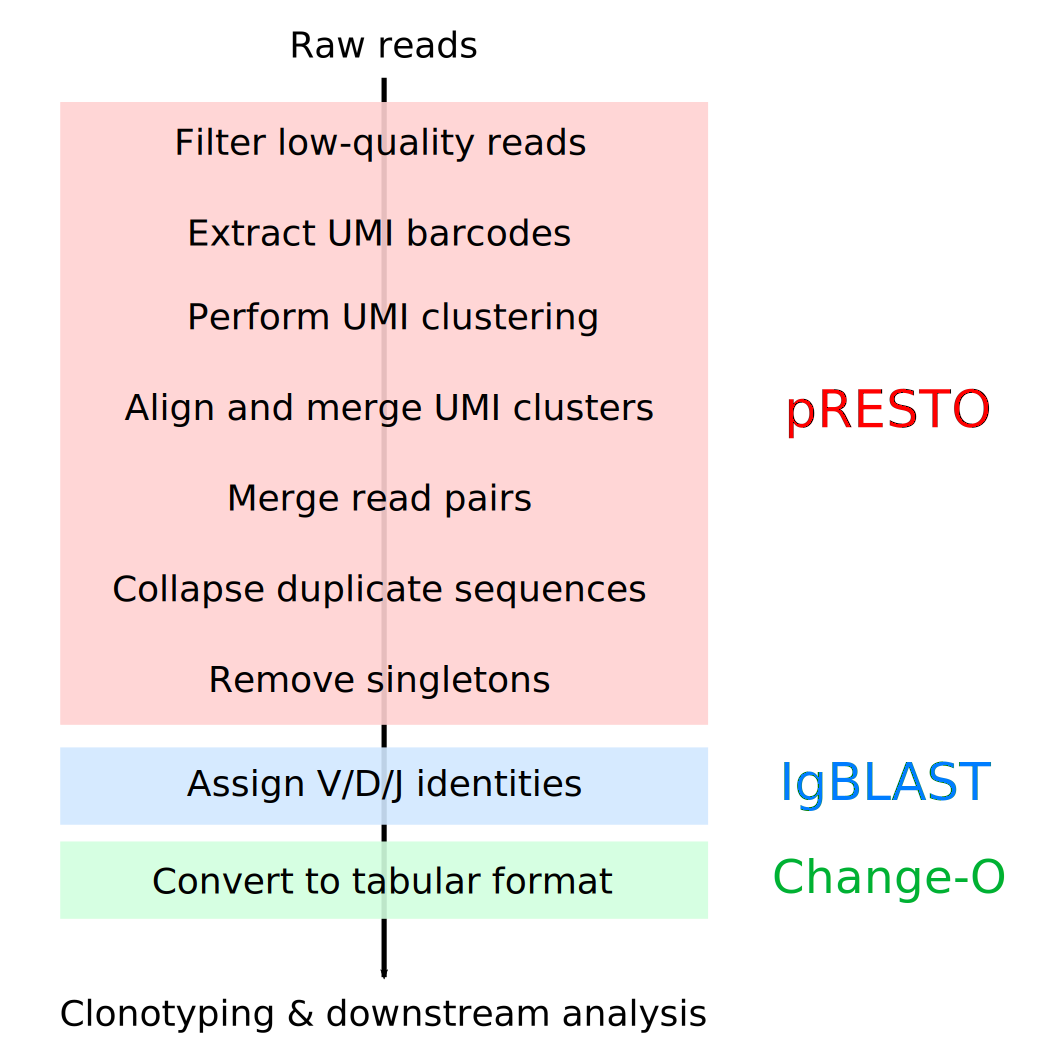
\includegraphics[width=0.6\textwidth]{_Figures/png_edited/igseq-preprocessing}
\vspace{0.5em}
\end{figure}

Raw \igseq data from the protocol described in \Cref{sec:igseq_protocol_library} takes the form of a large number of paired-end sequencing reads, each of which represents a partial, biased and error-prone sample from the set of input sequences in the original sample. To get from this fragmented and unreliable dataset to a set of complete, error-corrected and bias-adjusted \igh{} variable-region sequences, extensive pre-processing (\Cref{sec:methods_comp_igpreproc}) must be performed on the raw data. In this case, this pre-processing was largely carried out with \program{pRESTO} \parencite{vanderheiden2014presto}, part of the Immcantation suite of repertoire-sequencing analysis tools.

To begin with, each read pair in the dataset is annotated with various information about the source individual (ID, strain, sex, age and weight at death, etc.) as well as information about its place in the replicate structure of the experiment. The sequences are then filtered to remove low-quality sequences (with a mean Phred score of less than 20). % TODO: Citation for Phred score
Invariant primer sequences are trimmed from the ends of the reads, and the UMI sequence of each forward read (containing the TSA sequence) is extracted into a sequence annotation and removed from the read sequence.

As discussed in \Cref{sec:igseq_protocol_library}, the use of UMI sequences enables biases and errors in library insert sequences to be corrected by taking the consensus sequence of all reads sharing a given UMI. However, PCR and sequencing errors can also affect the sequence of the UMI itself, in which case reads that in fact belong to a single group will be spuriously separated during pre-processing; this can result in spuriously low UMI group sizes, spuriously high numbers of unique sequences, and avoidable loss of sequencing data due to reads with erroneous barcodes being discarded (as low-quality, low-read-count unique sequences) at various points in the pre-processing pipeline \parencite{shlemov2017igrec}. In addition to these barcode \textit{errors}, barcode \textit{collisions} can occur, in which multiple distinct sequences are labelled with the same UMI sequence and spuriously grouped together during UMI grouping. This can lead to spuriously large MIGs and spuriously low numbers of unique sequences, and in extreme cases lead to the rejection and loss of entire MIGs due to an insufficiently high level of sequence identity during consensus-read generation \parencite{shlemov2017igrec}.

In order to reduce the effect of such barcode errors and collisions on the pre-processing pipeline, primer-trimmed forward reads in this pipeline undergo clustering following extraction of UMI sequences. Firstly, reads are clustered by UMI sequence, and those with sufficiently similar UMIs are grouped together into a single cluster even if their UMIs differ slightly. Following this, read insert sequences within a given cluster are themselves clustered, and those with sufficiently different insert sequences are split apart into separate clusters. Following these clustering steps, each cluster consists of reads with highly similar barcode sequences as well as similar insert sequences; it is these clusters, rather than the raw UMI sequences, on which consensus-read generation is performed.

Following cluster inference as described above, annotations (including barcode and cluster annotations) are copied from each TSA-bearing forward-read to its mate among the reverse reads. The forward and reverse reads were then separately grouped by cluster identity and collapsed into a consensus sequence, based on the quality score of each aligned base call at each position \parencite{vanderheiden2014presto}. As most PCR and sequencing errors should be present in only a minority of the sequences descended from a given input sequence, this process effectively corrects these errors, while also removing the effect of biased amplification on observed sequence abundance. The more sequences present in a given cluster, the more effective is consensus-read generation at correcting these errors; as such, there is a trade-off inherent in the amount of oversequencing of the molecules in each library, with more oversequencing improving error correction but reducing the amount of data available \parencite{turchaninova2016igprep}.

Following consensus-read generation, pairs of forward and reverse consensus reads with matching cluster annotations are assembled into a single contiguous sequence, ideally covering the entire variable-region sequence of the template molecule; forward or reverse consensus reads lacking a mate in the other read set are discarded. At this point in the pipeline, each entry is assumed to represent a distinct RNA template molecule in the original sample. Sequences with different cluster annotations but matching insert sequences are then collapsed together into a single sequence, which is annotated with the number of contributing consensus reads; each sequence entry now represents a unique sequence in the dataset. Finally, unique sequences represented by only a single read pair (which could not be corrected by consensus-read generation and are therefore highly unreliable) are discarded.

At the end of the \program{pRESTO} pre-processing pipeline, the raw data has been processed into a set of complete variable-region sequences, each of which is annotated with the number of contributing reads and the number of distinct instances of that sequence found in the dataset. These sequences are then assigned V/D/J-identities through alignment to reference databases with \program{IgBLAST} \parencite{ye2013igblast}. Finally, the sequences and their metadata, including annotations and V/D/J-identities, are converted by \program{Change-O} (another program from the Immcantation suite) \parencite{gupta2015changeo} into tabular format for efficient downstream processing and analysis (\Cref{fig:igrace-preprocessing}).

\section{Establishing \igseq in turquoise killifish: pilot study}
\label{sec:igseq_pilot}

In order to refine and functionally validate the library-preparation protocol and processing pipeline described in \Cref{sec:igseq_protocol}, as well as assess the state of the turquoise-killifish antibody repertoire in mature adults, a group of four eight-week old adult male killifish from the second sample group described in \Cref{sec:igseq_samples} (specifically, fish 2-03, 2-04, 2-05 and 2-06 from \Cref{tab:igseq-cohorts-fish}) were selected for a pilot study. In this experiment, total RNA was isolated twice independently from each fish, and independent library preps were performed once on the first RNA isolate and twice on the second, for a total of three replicates per individual (\Cref{fig:igseq-pilot-design}). These twelve replicates were sequenced together in a single MiSeq run, yielding a total of \embed{_Figures/txt/pilot-reads-raw-total.txt} million read pairs (\embed{_Figures/txt/pilot-reads-raw-replicate-min.txt} to \embed{_Figures/txt/pilot-reads-raw-replicate-max.txt} million pairs per replicate, \embed{_Figures/txt/pilot-reads-raw-individual-min.txt} to \embed{_Figures/txt/pilot-reads-raw-individual-max.txt} million pairs per individual). These data were then used to develop the downstream analysis pipeline for killifish immunoglobulin-sequencing data, validate the performance and replicability of the protocol, and investigate the state of the antibody repertoire in mature adult killifish. % TODO: Cite appropriate subsections?

\begin{figure}
\centering
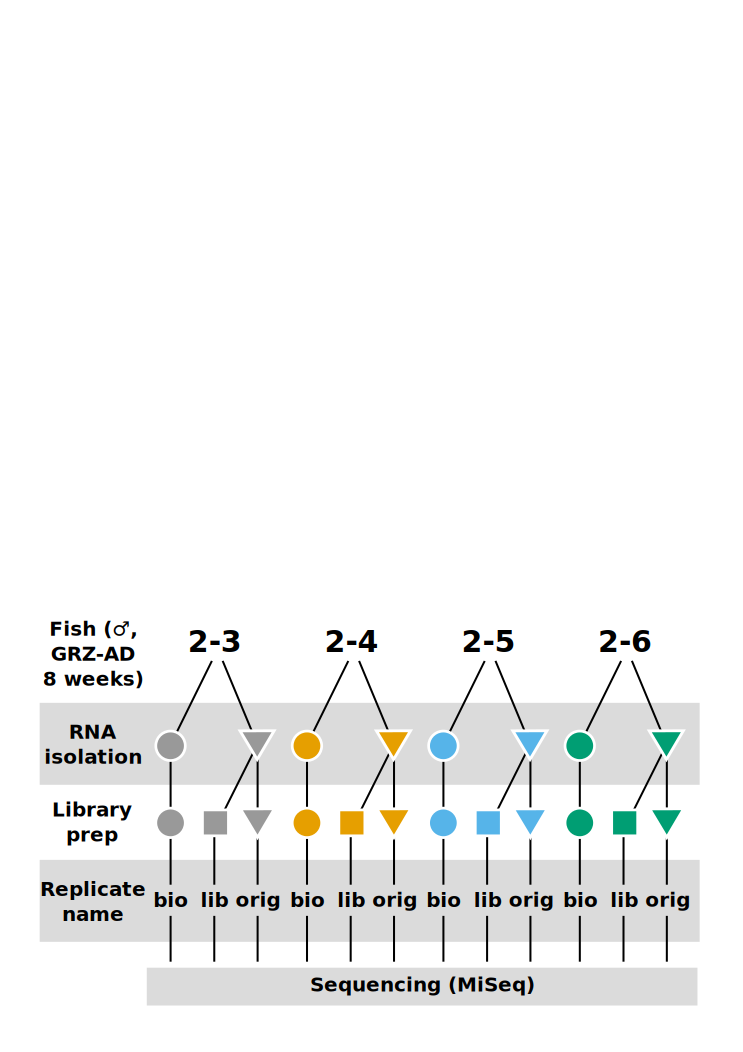
\includegraphics[width = 0.9\textwidth]{_Figures/png_edited/igseq-pilot-design_wide.png}
\caption{Experimental design of pilot study, showing relationship between replicates for each individual. Colour denotes individual of origin, while shape denotes replicate type.}
\label{fig:igseq-pilot-design}
\end{figure}

\subsection{Read survival and composition}
\label{sec:igseq_pilot_composition}

\Cref{fig:igseq-pilot-read-survival-init} shows the absolute and relative read survival for each of the twelve replicates throughout the pre-processing pipeline, up to and including VDJ assignment and Change-O table construction. The twelve replicates show relatively consistent behaviour, with \embed{_Figures/txt/pilot-read-survival-init-min.txt}\,\% to \embed{_Figures/txt/pilot-read-survival-init-max.txt}\,\% of reads surviving the entire process. Of those that do not, the biggest losses typically occur during quality filtering and removal of singleton sequences, with most other steps giving rise to relatively little sequence loss (\Cref{fig:igseq-pilot-read-survival-init-b}).

\begin{figure}
\centering
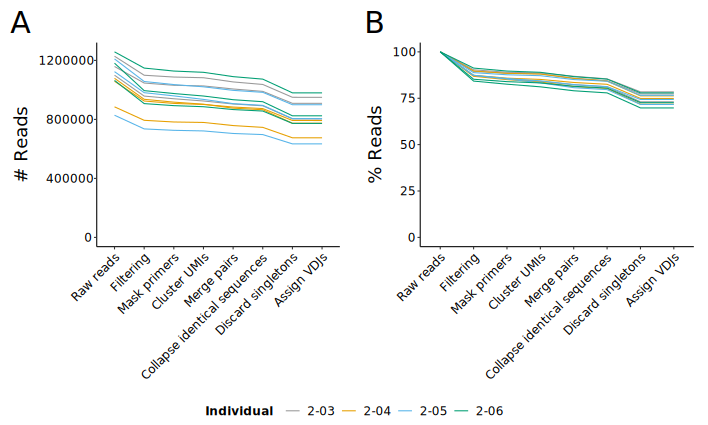
\includegraphics[width = 0.9\textwidth]{_Figures/png/pilot-read-survival-init.png}
\begin{subfigure}{0em}
\phantomsubcaption{}
\label{fig:igseq-pilot-read-survival-init-a}
\end{subfigure}
\begin{subfigure}{0em}
\phantomsubcaption{}
\label{fig:igseq-pilot-read-survival-init-b}
\end{subfigure}
\caption{Absolute (A) and relative (B) read survival during pre-processing of the pilot \igseq dataset, up to VDJ assignment and Change-O table construction.}
\label{fig:igseq-pilot-read-survival-init}
\end{figure}

In total, the pre-processed sequence repertoires of the pilot replicates contain between \embed{_Figures/txt/pilot-nseq-init-replicate-min.txt} and \embed{_Figures/txt/pilot-nseq-init-replicate-max.txt} unique sequences per replicate, corresponding to between \embed{_Figures/txt/pilot-nseq-init-individual-min.txt} and \embed{_Figures/txt/pilot-nseq-init-individual-max.txt} unique sequences per individual killifish and \embed{_Figures/txt/pilot-nseq-init-total.txt} unique sequences in total. Of these, \embed{_Figures/txt/pilot-nseq-init-pc-functional.txt}\,\% of sequences (corresponding to \embed{_Figures/txt/pilot-nreads-init-pc-functional.txt}\,\% of sequencing reads) are annotated by \program{Change-O} as functional, meaning they have successfully been assigned V- and J-identities, their V- and J-sequences are in-frame, and they do not contain any STOP codons (\Cref{fig:igseq-pilot-functional-prop-a}). A further \embed{_Figures/txt/pilot-nseq-init-pc-noj.txt}\,\% of sequences (corresponding to \embed{_Figures/txt/pilot-nreads-init-pc-noj.txt}\,\% of reads) failed to be assigned even an uncertain J-identity, meaning that no \jh sequence in the reference database aligned to the insert sequence; the remaining \embed{_Figures/txt/pilot-nseq-init-pc-other.txt}\,\% of sequences (corresponding to \embed{_Figures/txt/pilot-nreads-init-pc-other.txt}\,\% of reads) have a J-assignment but are rendered nonfunctional by an internal STOP codon and/or a frameshift between their V- and J-sequences (\Cref{fig:igseq-pilot-functional-prop-a}).

\begin{figure}
\centering
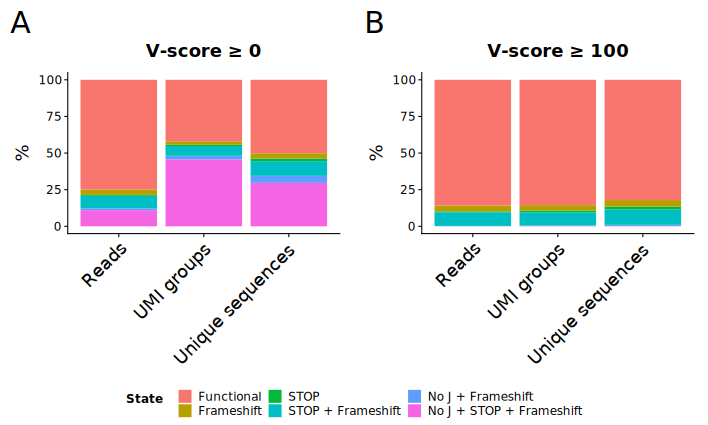
\includegraphics[width = 0.9\textwidth]{_Figures/png/pilot-functional-prop}
\begin{subfigure}{0em}
\phantomsubcaption{}
\label{fig:igseq-pilot-functional-prop-a}
\end{subfigure}
\begin{subfigure}{0em}
\phantomsubcaption{}
\label{fig:igseq-pilot-functional-prop-b}
\end{subfigure}
\caption{Proportion of input reads, UMI groups and unique sequences in the pilot \igseq dataset belonging to different (non)functional categories, before (A) and after (B) filtering on V-alignment score.}
\label{fig:igseq-pilot-functional-prop}
\end{figure}

As genuinely recombined but nonfunctional sequences would be expected to have undergone V(D)J recombination and so have a complete J-sequence, the lack of assigned J-identities for a significant minority of sequences suggests that this subset of sequences may be artefactual, erroneous or otherwise malformed. Supporting this assumption, sequences without J-assignments overwhelmingly have very low V-alignment scores reported by \program{IgBLAST}, with an average score of \embed{_Figures/txt/pilot-vscore-mean-noj.txt} $\pm$ \embed{_Figures/txt/pilot-vscore-sd-noj.txt} (mean $\pm$ standard deviation), compared to \embed{_Figures/txt/pilot-vscore-mean-other.txt} $\pm$ \embed{_Figures/txt/pilot-vscore-sd-other.txt} for other nonfunctional sequences and \embed{_Figures/txt/pilot-vscore-mean-functional.txt} $\pm$ \embed{_Figures/txt/pilot-vscore-sd-functional.txt} for functional sequences (\Cref{fig:igseq-pilot-functional-vscores}). A simple V-score cut-off of 100, therefore, effectively removes the vast majority of these low-quality sequences, while leaving the population of functional sequences intact (\Cref{fig:igseq-pilot-functional-prop-b}).

\begin{figure}
\centering
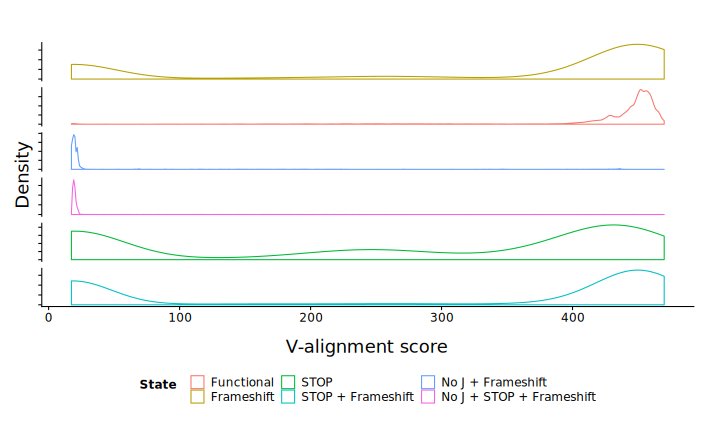
\includegraphics[width = 0.9\textwidth]{_Figures/png/pilot-functional-vscores}
\caption{Kernel density plots of distributions of V-alignment scores among unique sequences in the pilot \igseq dataset. Vertical axes are not to scale between sequence categories.}
\label{fig:igseq-pilot-functional-vscores}
\end{figure}

In total, \embed{_Figures/txt/pilot-nseq-init-dropped-vscore.txt} unique sequences, corresponding to \embed{_Figures/txt/pilot-read-survival-rel-loss-total.txt}\,\% of input reads, were removed in this way. As a result, including this final filtering step, between \embed{_Figures/txt/pilot-read-survival-all-min.txt}\,\% and \embed{_Figures/txt/pilot-read-survival-all-max.txt}\,\% of reads per input library survived the complete pre-processing process (\Cref{fig:igseq-pilot-read-survival-all}), a good range suggesting both that the library-preparation protocol successfully captured antibody-repertoire sequencing data from turquoise killifish for the first time, and that the subsequent computational pipeline was able to completely and successfully process the majority of the resulting data. Of the remaining \embed{_Figures/txt/pilot-nseq-init-kept-vscore.txt} unique sequences present in the dataset, \embed{_Figures/txt/pilot-nseq-init-functional-filtered.txt} (\embed{_Figures/txt/pilot-nseq-init-pc-functional-filtered.txt}\,\%) are functional, \embed{_Figures/txt/pilot-nseq-init-other-filtered.txt} (\embed{_Figures/txt/pilot-nseq-init-pc-other-filtered.txt}\,\%) are rendered nonfunctional by a STOP codon or frameshift, and only \embed{_Figures/txt/pilot-nseq-init-noj-filtered.txt} (\embed{_Figures/txt/pilot-nseq-init-pc-noj-filtered.txt}\,\%) could not be assigned a J-identity (\Cref{fig:igseq-pilot-functional-prop-b}). These results confirm that the data from this first \igseq experiment in the turquoise killifish are of sufficient quality to proceed to clonotyping and analysis of repertoire diversity.

\begin{figure}
\centering
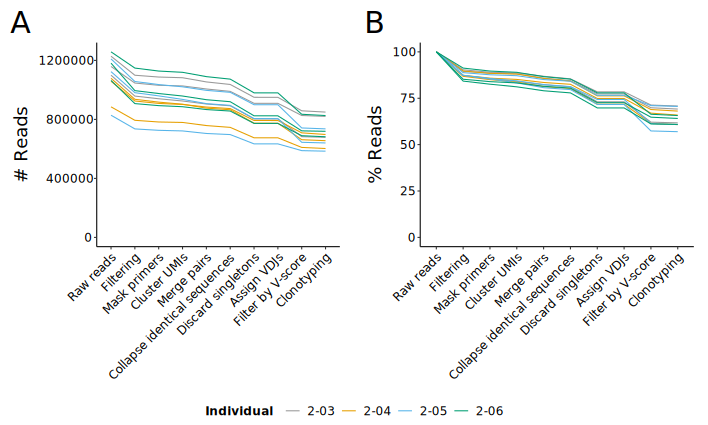
\includegraphics[width = 0.9\textwidth]{_Figures/png/pilot-read-survival-all.png}
\begin{subfigure}{0em}
\phantomsubcaption{}
\label{fig:igseq-pilot-read-survival-all-a}
\end{subfigure}
\begin{subfigure}{0em}
\phantomsubcaption{}
\label{fig:igseq-pilot-read-survival-all-b}
\end{subfigure}
\caption{Absolute (A) and relative (B) read survival during pre-processing of the pilot \igseq dataset, up to and including clonotyping.}
\label{fig:igseq-pilot-read-survival-all}
\end{figure}

\subsection{Clonotyping and clonal repertoire diversity}
\label{sec:igseq_pilot_clones}

Following assignment of VDJ identities and quality filtering, sequences in an antibody repertoire can be assigned to clones: groups of B-cells descended from a single \naive B-cell ancestor, and therefore sharing a single VDJ-recombination event. Sequences in the same clone are said to share a \textit{clonotype}. In \program{Change-O}, clonotyping is performed by dividing sequences into groups sharing a consistent V-assignment, J-assignment and CDR3 length, then performing single-linkage clustering on each group of sequences based on Hamming distances between CDR3 sequences \parencite{gupta2017hierarchical}. To identify a distance threshold for cutting the cluster dendrogram into clones, each unique sequence in the repertoire is assigned a nearest-neighbour distance based on the length-normalised Hamming distance to the most similar sequence in the repertoire. The resulting nearest-neighbour distance is typically bimodal, with the lower peak (representing more-similar sequences) indicating members of the same clonotype and the higher peak (representing less-similar sequences) indicating members of different clones; by fitting a pair of gamma or normal distributions to these two peaks, a distance threshold for clonotype membership can be determined according to the desired levels of sensitivity and specificity \parencite{nouri2018threshold} (\Cref{sec:methods_comp_igpreproc_clones}). By cutting the cluster dendrogram at this threshold, each group of repertoire sequences can be separated into some number of distinct clones, each of which shares a unique \naive B-cell ancestor.
% TODO: Figure describing clonotyping process

One disadvantage of single-linkage clustering in this context is that non-informative \sequence{N} positions can result in artifactual links between unrelated sequences. As such, sequences with a large number of junctional \sequence{N} positions can significantly disrupt the clonotyping process. On the other hand, as over \embed{_Figures/txt/pilot-filtered-nn-any.txt}\,\% of unique sequences in the pilot dataset contain at least one such junctional \sequence{N} position, excluding them all would represent a significant loss of data. In order to minimise the number of discarded sequences while also minimising the disrupting effects of sequences with junctional \sequence{N}s, sequences with exactly one junctional \sequence{N} position (comprising \embed{_Figures/txt/pilot-filtered-1n-total.txt}\,\% of total sequences and \embed{_Figures/txt/pilot-filtered-1n-withn.txt}\,\% of sequences with at least one junctional \sequence{N}; \Cref{tab:igseq-pilot-filtered-nn}) were included in the clonotyping process for the pilot dataset, while those with two or more junctional \sequence{N} positions were excluded. This procedure successfully assigned clonal identities to \embed{_Figures/txt/pilot-nseq-assigned-clones.txt}\,\% of unique sequences in the V-score-filtered dataset, with fewer than \embed{_Figures/txt/pilot-nseq-lost-clonotyping.txt} sequences (corresponding to \embed{_Figures/txt/pilot-pc-reads-lost-clonotyping.txt}\,\% of input reads) lost during the clonotyping phase of the pipeline.

\begin{table}
\caption{Distribution of junctional \sequence{N} positions in the V-score-filtered pilot dataset.}
\label{tab:igseq-pilot-filtered-nn}
% latex table generated in R 3.5.2 by xtable 1.8-3 package
% Wed Apr  3 14:27:33 2019
\begin{tabular}{lrrr}
  \toprule \# junctional Ns & \# unique sequences & \% of all sequences & \% of sequences with $>$0 junctional Ns \\ 
  \midrule 0 & 49134 & 88.924 & 0.00 \\ 
  1 & 3388 & 6.132 & 67.94 \\ 
  2 & 961 & 1.739 & 19.27 \\ 
  3 & 324 & 0.586 & 6.50 \\ 
  4 & 125 & 0.226 & 2.51 \\ 
  5 & 93 & 0.168 & 1.86 \\ 
  $>$5 & 96 & 0.174 & 1.93 \\ 
   \bottomrule \end{tabular}

\end{table}

In total, \embed{_Figures/txt/pilot-nclones-individual-min.txt} to \embed{_Figures/txt/pilot-nclones-individual-max.txt} clones were identified per individual fish in the pilot dataset. As expected, the clone-size distribution is overwhelmingly dominated by small clones (\Cref{fig:igseq-pilot-clone-sizes-sizes}): across all individuals, \embed{_Figures/txt/pilot-nclones-pc-1count.txt}\,\% of clones are observed as just a single unique sequence across all replicates, while \embed{_Figures/txt/pilot-nclones-pc-small.txt}\,\% contain fewer than five unique sequences. As a result, the great majority of clones (\embed{_Figures/txt/pilot-nclones-pc-1rep.txt}\,\%) are observed in only a single replicate per individual, with \embed{_Figures/txt/pilot-nclones-pc-2rep.txt}\,\% present in two replicates and only  \embed{_Figures/txt/pilot-nclones-pc-3rep.txt}\,\% shared across all three. Unsurprisingly, however, larger clones are much more likely to be shared across multiple replicates (\Cref{fig:igseq-pilot-clone-sizes-reps}), consistent with a model in which a very large number of small clones are sampled only rarely while a much smaller number of large clones is sampled much more often. % TODO: Cite Walczak diversity paper here
Overall, the level of agreement between the replicates is high (\Cref{fig:igseq-pilot-clone-sizes-cor-boxplots,fig:igseq-pilot-clone-sizes-cor-scatter}), with an average inter-replicate correlation in clone size of $r=\embed{_Figures/txt/pilot-clone-sizes-cor-avg.txt}$, indicating that, despite the problem of undersampling many very small clones, the clonal composition of the killifish can be captured reproducibly by \Igseq.

\begin{figure}
\centering
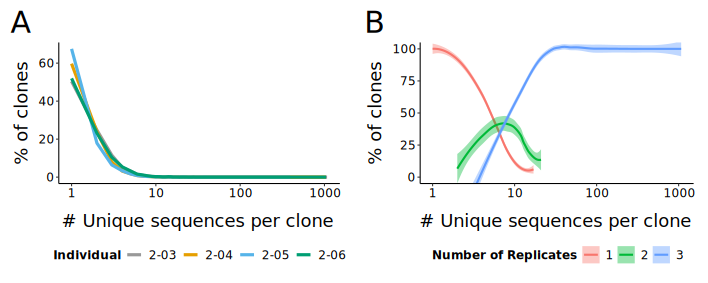
\includegraphics[width = 0.9\textwidth]{_Figures/png/pilot-clone-sizes}
\begin{subfigure}{0em}
\phantomsubcaption{}
\label{fig:igseq-pilot-clone-sizes-sizes}
\end{subfigure}
\begin{subfigure}{0em}
\phantomsubcaption{}
\label{fig:igseq-pilot-clone-sizes-reps}
\end{subfigure}
\caption{(A) Proportion of clones of different sizes for each individual in the pilot dataset, measured in unique sequences per clone. (B) Proportion of clones of each size found across one, two or all three replicates of the appropriate individual.}
% TODO: Add suitable overall figure title
\label{fig:igseq-pilot-clone-sizes}
\end{figure} % TODO: Correct subplot B legend spacing; describe smoothing plot better

\begin{figure}
\centering
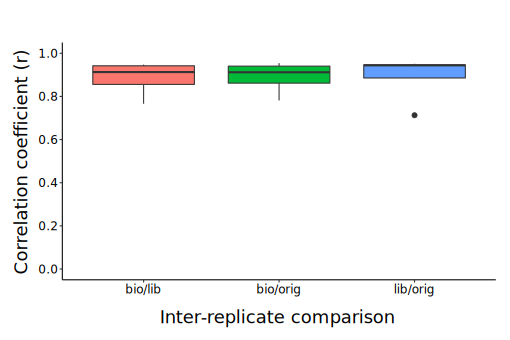
\includegraphics[width = 0.7\textwidth]{_Figures/png/pilot-clone-sizes-cor-boxplots}
\caption{Boxplots showing distribution of Pearson's product-moment correlation coefficients of clone sizes for each pair of replicates, as measured by the number of unique sequences per clone in each replicate. Clones absent in a given replicate were given a size of zero.}
% TODO: Add suitable overall figure title
\label{fig:igseq-pilot-clone-sizes-cor-boxplots}
\end{figure}

\begin{figure}
\centering
\includegraphics[width = 0.7\textwidth]{_Figures/png/pilot-clone-sizes-cor-scatter}
\caption{Scatter plots comparing clone sizes across biological replicates for each individual in the pilot dataset.}
% TODO: Add suitable overall figure title
\label{fig:igseq-pilot-clone-sizes-cor-scatter}
\end{figure}

